\chapter{Systemdesign und Implementierung}
\section{Systemübersicht}
\begin{figure}[!h]
	\centering
   	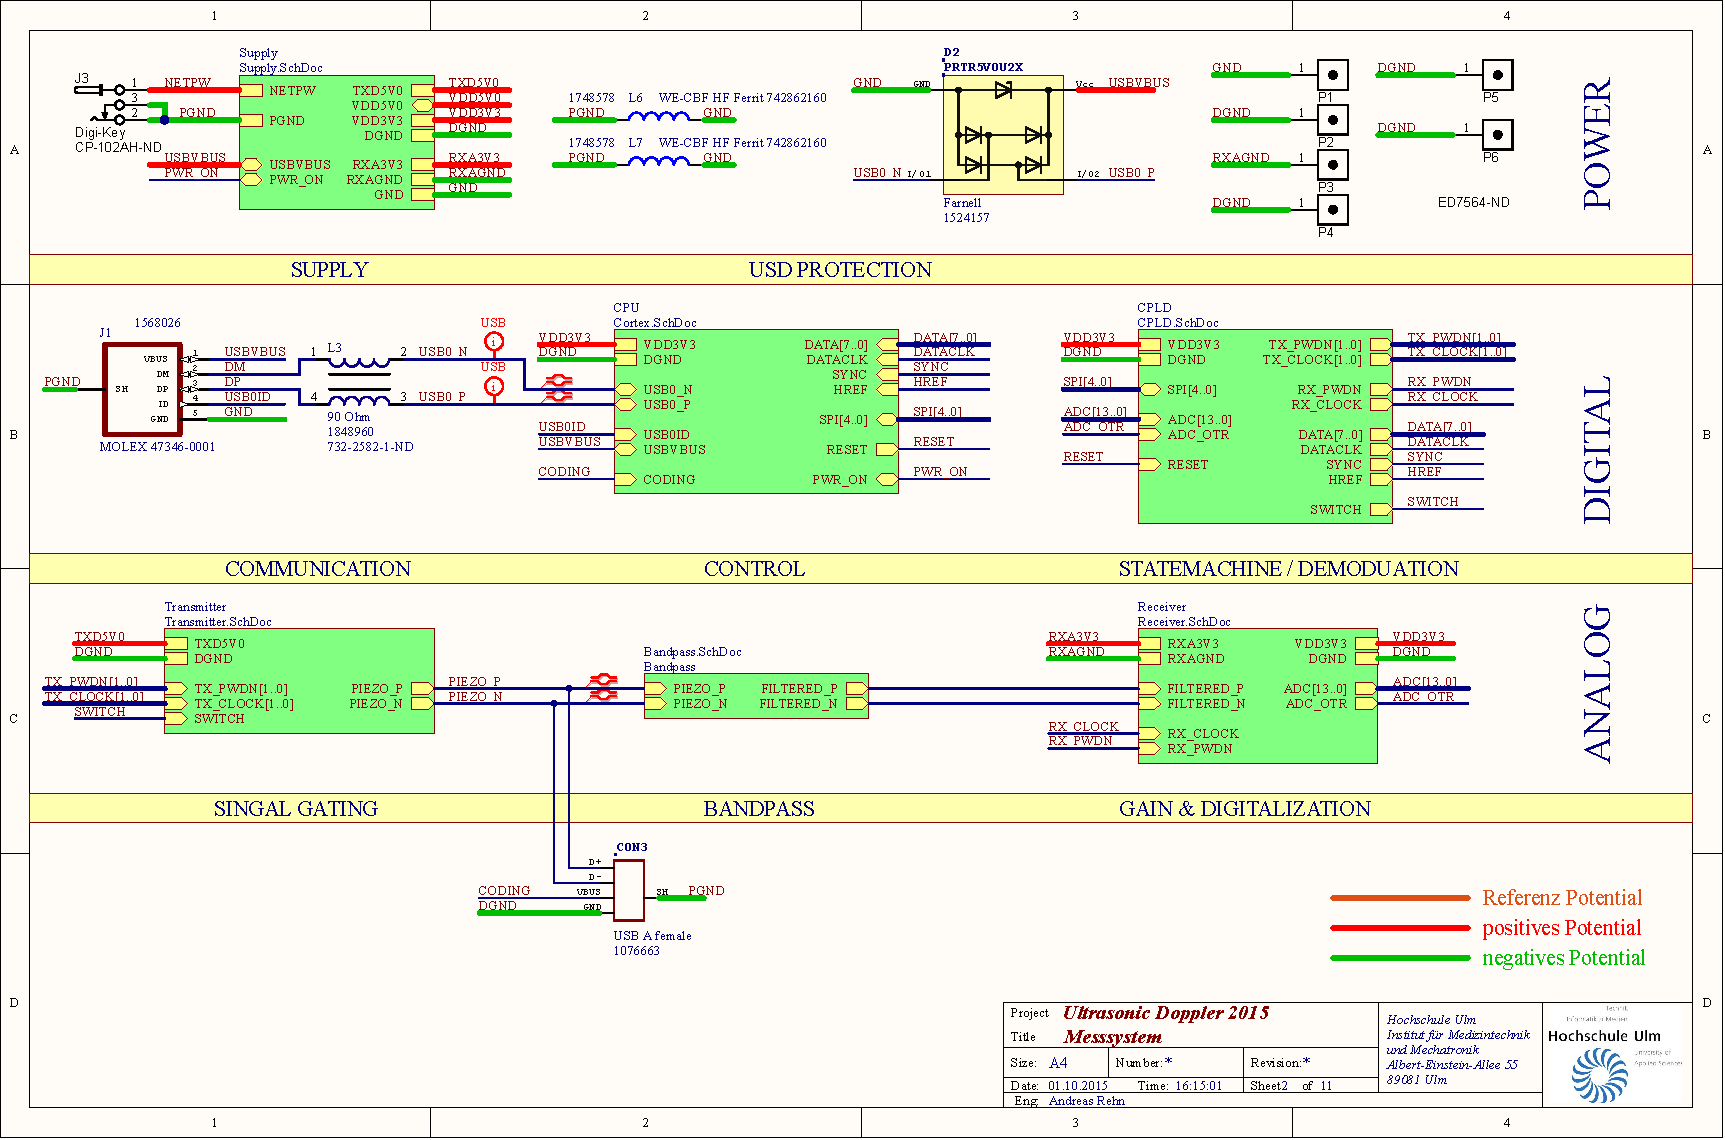
\includegraphics[page=1,width=1.0\textwidth, trim= 5mm 5mm 5mm 5mm, clip=true]{images/pcb/new.PDF}%docu
    \caption{Modulübersicht des Systems ohne mechanische und externe Komponenten}
    \label{fig:system}
\end{figure}
In diesem Kapitel wird das erstellte System und dessen Module näher beschrieben. Dabei wird das System in Analog, Digital, Power und mechanische Komponenten untergliedert.
\begin{itemize}
\item Um das System mit Energie zu versorgen wird eine Stromquelle benötigt, welche in \autoref{sec:supply} beschrieben wird. Da das System für die medizinische Anwendung konzipiert ist, wird zudem die Einspeisung des Systems und des \ac{pc}s des Benutzers beschrieben. Diese Beschreibung ist notwendig, da die Spannungsversorgung des Systems auf dem Verhalten der Einspeisung aufbaut.
\item Das Modul Analog beinhaltet dabei den Transmitter, welcher das zu emittierende Signal generiert, sowie den Receiver, welcher aus einen Bandpassfilter, einer \ac{lna} und einer Digitalisierung besteht.
\item Das Modul Digital beinhaltet hingegen die Ansteuerung des Transmitters und des Receivers sowie die Demodulierung und den Datentransfer zwischen dem System und den \ac{pc} des Nutzers.
\item Das Modul Gehäuse wurde aus der Übersicht entfernt, da dieses das gesamte Messsystem beinhaltet und nur die Schnittstellen für die Anbindung der Sonde, des \ac{pc}s sowie der Stromversorgung zur Verfügung stellt. Aus diesem Grund wurde das Gehäuse zwar vorgesehen, jedoch geht dieses in der aktuellen Entwicklungsphase nicht in die Implementierung des Systems ein.
\end{itemize}
Nachfolgend werden die genannten Module mit Spannungsversorgung, Kommunikation, Steuerung / Demodulierung, der Transmitter, der Receiver mit Bandpass sowie das Gehäuse näher betrachtet sowie erklärt. Zudem werden Aussagen über die Auslegung und die Realisierung dieser Module getroffen um den Leser ein besseres Verständnis des Systems und dessen Umsetzung zu geben.
\section{Spannungsversorgung}\label{sec:supply}
Damit das System arbeiten kann, benötigt das System elektrische Energie welche typischerweise von Außen zugeführt wird. Da der Fokus dieser Arbeit nicht auf der Energieversorgung des Dopplersystems liegt, wurde als Ausgangsbasis ein externes Schaltnetzteil der Firma SL Power Electronics verwendet, welches bei 230 V AC Netzspannung ein 19 V DC Ausgangsspannung mit 3,1 A liefert. Zudem ist das Netzteil GXM60-19A04 nach EN60601 geprüft und somit für medizinische Anwendungen zugelassen. Versionen für den internen Einbau sind dabei im Bereich von 5 bis 56 V DC beziehbar.\\%http://www.slpower.com/products/internal-medical-power-supplies/overview.html
Um elektromagnetische Störungen im System möglichst gering zuhalten, wurden Potentiale anhand der Arbeitsbereiche der elektronischen Komponenten bestimmt, festgelegt und gruppiert. Dabei ergab sich ein Potential für die digitale Signalverarbeitung, ein separiertes Potential für die analoge Signalverarbeitung sowie ein Potential für die Ansteuerung des Piezoelementes. Für die Potentiale wurden folgende Spannungen - 5 V DC \textit{TXD5V0} für die Piezoelementansteuerung, 3,3 V DC \textit{RXA3V3} für die analoge Signalverarbeitung und 3,3 V DC \textit{VDD3V3} für die digitale Signalverarbeitung - definiert.\\
Für die elektrische und mechanische Verbindung zwischen externen Schaltnetzteil und dem System wurde eine DC Power Jack Buchse gewählt, da das Netzteil geprüft ist und somit nicht veränderbar ist, ohne folgende Prüfungen und somit Kosten zu verursachen. Dabei ist bekannt, dass es zu Fehlbedienungen durch den Nutzer kommen kann, indem dieser Netzteile mit vertauschter Polung und oder Netzteile mit zu hohem Spannungsbereich nutzt. 
Für den Verpolungsschutz wurde ein kostengünstiger P-\ac{mosfet} genutzt, welcher nur durchschaltet, wenn das richtige Spannungspotenzial anliegt. Dieser limitiert gleichzeitig die minimale und maximale Spannung des Eingangs durch seinen Arbeitsbereich von \ac{ca} -0,55 V  bis -20 V DC. Dieser dient gleichzeitig als \textit{schwächstes} Bauelement, wenn der maximale Spannungsbereich überschritten wird, was die Fehlersuche beträchtlich einschränkt und folgende Komponenten schützt. Jedoch muss der \ac{mosfet} anschließend ausgetauscht werden.\\
Da das System auch über eine \ac{usb} Verbindung verfügt, kann das System theoretisch über eine \ac{usb} 2.0 Verbindung eine Spannung von 5 V DC mit einen maximalen Strom von 500 mA beziehen. Jedoch schwankt die unregulierte Spannungsversorgung je nach Quelle (\ac{zb}Laptop / \ac{pc}) von 4,75 V DC bis 5,5 V DC was für das Potential der Piezoelementansteuerung als nicht nutzbar erscheint. Zudem ist die erhöhte Stromaufnahme von 400 mA des Transmitters (\autoref{sec:transmitter}) nicht sichergestellt, wenn ein \ac{usb}-Hub oder mehrere Geräte an den \ac{pc} oder Laptop angeschlossen sind. Somit wurde eine Versorgung des Transmitters über \ac{usb} ausgeschlossen, jedoch können die analoge und die digitale Signalverarbeitung mit dieser Versorgung betrieben werden, was in dieser Phase der Entwicklung sinnvoll erscheint.
\subsection*{19 V DC zu 5 V DC}
Wie in \autoref{sec:transmitter} beschrieben, wird eine 5 Volt DC Spannung und ein 400 mA Strom für die Ansteuerung des Piezoelementes benötigt, damit ein Strom-Spannungswandler das zu emittierende Signal an die Amplitude des Piezoelementes anpassen kann. Um die benötigte Spannungspotential von 5 V DC zu genieren wurde der step-down (buck) Konvertierer MIC4680 der Firma MICREL genutzt, welcher einen maximalen Ausgangsstrom von 1,3 A liefern kann. Dieser arbeitet mit einer festen Frequenz von 200 \ac{khz} und besitzt einen Überstromschutz sowie eine automatische Abschaltung bei Übertemperatur.\\
Zudem wurde ein \ac{emi} Filter ausgelegt, welcher laut Simulation bei 75 \ac{khz} eine Dämpfung von -16 dB besitzt. Somit sollte eine ausreichende Dämpfung vorhanden sein, um die Oberwellen des Schaltreglers zu filtern und nicht in das Netz bzw. an das Netzteil einzukoppeln. Gleichzeitig kann durch dieses Filter eine Störfestigkeit gegen einstrahlende Frequenzen erreicht werden. % mit einer Dämpfung von -40 dB ab \ac{ca} 1 \ac{mhz}.
Da ein Schaltregler ein erhöhtes Rauschen aufweist, ist die Ausgangsspannung selbst durch Siebung und Glättung mit einen Kondensator nicht ideal für die Ansteuerung des Piezoelementes. Daher ist ein ADP7104 \ac{ldo} der Firma Analog Devices mit 550 mV dropout bei 500 mA vorgesehen, welcher ein Rauschen von 15 $\mu$V rms aufweist. Somit besteht die 5 Volt DC Generierung aus einen step-down, welcher die 19 V DC auf ein \ac{ca} 6,5 V DC Potenzial konvertiert mit einen nachgeschalteten \ac{ldo}. Somit kann eine Reduzierung der thermischen Belastung der Platine erreicht werden, was zudem auch den realen Leistungsbedarf senkt.\\
Parallel zu der Transmitterversorgung ist der analoge Leistungsschalter TPS2115A der Firma Texas Instruments verbaut, welcher automatisch die Stromversorgung der analogen und digitalen Signalverarbeitung von \ac{usb} auf das externe Netzteil schaltet, wenn Dieses angeschlossen ist. Somit kann sichergestellt werden, dass die \ac{pc} Software den aktuellen Stand des Systems an den Nutzer aufbereitet wiedergeben kann.
\subsection*{5 V DC zu 3,3 V DC analog}
Bei mixed-Signal \ac{pcb} Layouts muss auf Stromschleifen geachtet werden. Zudem wurde sich dafür entschieden, dass die Potenziale für die analoge und digitale Signalverarbeitung getrennt werden, was unterschiedliche Masseflächen mit Sternpunktverbindung zur Folge hat. Zudem war bei Erstellung des Layouts die maximale Taktfrequenz der analogen Komponenten durch die Digitalisierung mit 64 \ac{msps} limitiert.\\
Um die \ac{ic}s der analogen Signalverarbeitung zu stabilisieren sowie voneinander zu entkoppeln wurde jeweils ein Tiefpass 2. Ordnung vorgesehen. Dieser besitzt einen parallel geschalteten Pufferkondensator, welcher den Strom schnell an das Bauelement abgeben kann, und eine in Reihe geschaltete Spule, welche den Strom für die Aufladung des Kondensators begrenzt. Dadurch wird der \ac{ldo} weniger dynamisch belastet, wodurch ein stabiler Spannungspegel sichergestellt werden kann. Für die Generierung der 3,3 V DC Spannung wurde der \ac{ldo} ADP151 der Firma Analog Devices gewählt, da dieser 200 mA bei einen Spannungsripple von 9 $\mu$V rms liefern kann. Somit ist dieser ideal geeignet für die Versorgung der analogen Bauelemente.
%
%ref auf münzner
%
\subsection*{5 V DC zu 3,3 V DC digital}
Für die Versorgung des \ac{cpld}s und des ARM\SymbReg Cortex\SymbReg-M wurde der \ac{ldo} ADP7104 der Firma Analog Devices verwendet. Dieser liefert 500 mA bei einen Spannungsripple von 15 $\mu$V rms.
\newpage
\section{Transmitter}\label{sec:transmitter}
%scr0004 -> 10 Ohm Last
%scr0006 -> 8 Ohm Last
%scr0007 -> 6 Ohm Last
\newpage
\section{Entkopplung Transmitter Receiver}
Um das Verhalten von Transmitter und Receiver zu Entkoppeln wurden antiparallele Dioden (BAT64-04) verwendet. Die Durchbruchspannung dieser Dioden liegt bei 40 Volt, welche weder vom Trägersignal, noch vom empfangen Signal erreicht werden. Somit können die Dioden als Richtungsbegrenzer angesehen werden und das Verhalten kann für die Entkopplung genutzt werden. Ab 0,3 Volt Vorwärtsspannung hingegen werden diese leitend \ac{bzw} weisen diese ein niederohmiges Verhalten auf, woraufhin die Spannung durch die Anordnung der Dioden auf rund $\pm$ 0,3 Volt limitiert wird.\cite{bat64}
\begin{description}
\item[Senden des Signals:] Um den Receiver bei der Übertragung des Burstsignals durch die hohen Amplituden nicht zu zerstören wird das niederohmige Verhalten antiparalleler Dioden genutzt. Dabei sieht das Netzwerk einen niederohmigen Verbraucher, wodurch mögliche Ströme primär über die Dioden fließen und der Spannungspegel auf rund $\pm$ 0,3 Volt begrenzt wird. Je nach Positionierung im Netzwerk können Bauelemente und deren Verhalten verwendet oder terminiert werden. In dieser Arbeit wurden die antiparallelen Dioden nach den Induktivitäten des Bandpassfilters des Receiver Moduls positioniert, wodurch die Breitbandigkeit der Sonde gesteigert wird.
\item[Empfang des Signals:] In dieser Phase soll das Netzwerk nur den Receiver sehen. Da mit Empfangssignalen zu rechen ist, die kleiner $\pm$ 0,3 Volt sind, kann der Transmitter durch eine Serienschaltung der antiparallelen Dioden entkoppelt werden. Aus diesen Grund kann ein Widerstand zwischen Transmitter und den Dioden genutzt werden, um die Ausschwingzeit des Kristalls zu reduzieren, jedoch das Signal nicht beim Empfang belastet.
\end{description}
\begin{figure}[!h]
        \centering
        \begin{subfigure}[b]{0.48\textwidth}
        \centering
                \includegraphics[page=11, width=0.8\textwidth, trim =242mm 80mm 10mm 87mm, clip=true]{images/pcb/docu.pdf}
	    		\caption{im Ausgang der Transmitterschaltung}
	    		\label{fig:dioden_tx}
        \end{subfigure}%
        \hfil
        ~ %add desired spacing between images, e. g. ~, \quad, \qquad, \hfill etc.
          %(or a blank line to force the subfigure onto a new line)
        \begin{subfigure}[b]{0.48\textwidth}
                \includegraphics[page=3, width=\textwidth, trim=50mm 91mm 150mm 59mm, clip=true]{images/pcb/new.pdf}
		    \caption{im Bandpassfilter der Recieverschaltung}
		    \label{fig:dioden_rx}
        \end{subfigure}
        \caption{Anordnung der Dioden}\label{fig:filter_final}
\end{figure}
\newpage
\section{Receiver}\label{sec:receiver}
Der Receiver dient für den Empfang der \ac{rf} Signale sowie deren analogen Aufbereitung, damit diese Signale ideal digitalisiert werden können.\\
Dabei besteht das Receiver Modul des Systems aus einen differenziellen analogen Bandpass 2. Ordnung für die grundlegende Rauschminimierung der eingekoppelten und unerwünscht generierten Signale, einen Vorverstärker, welcher die gefilterten Signalamplituden an den Eingangsbereich des \ac{adc} Wandlers anpasst, sowie einen nachfolgenden \ac{adc} Wandler mit vorgeschalteter Impedanzanpassung.\\
In diesem Kapitel werden die einzelnen Abschnitte des Receiver Moduls näher beschrieben.
\subsection{Analoger Bandpass}
Wie in \autoref{sec:receiver} beschrieben, wird ein analoger Bandpass benötigt, um unerwünschte Signale zu dämpfen und somit das Rauschen zu minimieren. Dafür musste das Arbeitsfrequenzband definiert und der analoge Bandpass beschrieben werden.\\
Da das Arbeitsfrequenzband des Filter grundsätzlich beschreibt, werden die zu emittierenden Frequenzen (2, 4, 8 \ac{mhz}) in die Charakteristik einbezogen. Des weiteren soll der Dopplereffekt genutzt werden, welcher in \autoref{sec:dopplereffekt} auf Seite \pageref{sec:dopplereffekt} beschrieben ist. Dabei ist zu beachten, dass die Frequenz des emittierten Signales um bis zu \ac{ca} $\pm$ 10 \ldots 20 \ac{khz} verschoben werden kann. Außerdem muss beachtet werden, dass der Burst bei längerer Laufzeit einer erhöhten Dämpfung unterliegt. Somit muss das zeitliche Verhalten der emittierten Welle genauer betrachtet werden, da Reflektionen an Impedanzänderungen bzw. Dichteänderungen (Zellwände) auftreten und ein statisches Echo, also eine Reflektion ohne Frequenzänderung, zur Folge haben. Des weiteren unterliegt das Ein- und Ausschwingverhalten des Piezoelementes physikalischen Regeln, welche exponentiell sind\textbf{[REF!]}. Somit wird durch das Verhalten des Piezoelements das Trägersignal niederfrequent überlagert, was sich durch die \ac{prf} zyklisch wiederholt. Auch kann nicht ausgeschlossen werden, dass Oberwellen des Trägersignals gebildet und reflektiert werden. Da gerade Oberwellen durch den nachgestellten digitalen \ac{fir} Tiefpassfilter eliminiert werden können sind diese vernachlässigbar. Jedoch können ungerade Oberwellen ein summarischen Offset bei der Demodulierung erzeugen, welche die Messwerte verfälschen können. Dieses Verhalten gilt für alle Trägerfrequenzen.\\
Aus den oben genannten Fakten ist zu schlussfolgern, dass eine Hoch- und eine Tiefpass benötigt wird, um das Breitbandrauschen zu reduzieren und die Trägerfrequenzen mit dessen Dopplerschiebefrequenzen ungedämpft passieren zu lassen. Dabei sollte ein Hochpass für das Ausschwingverhalten des Piezoelementes und ein Tiefpass für die unerwünschten Oberwellen der Trägerfrequenzen dimensioniert werden.\\
Ein Bandpass zweiter Ordnung\footnote{40 dB/Dekade} wurde daher in Betracht gezogen, wobei die untere Grenzfrequenz $f_L$ auf 100 \ac{khz} und die obere Grenzfrequenz $f_H$ auf 8 \ac{mhz} festgelegt wurde. Zudem soll die minimale Dämpfung im Bereich von 2 \ac{mhz} liegen, da diese Trägerfrequenz die längste Laufzeit besitzt.
\subsection*{Implementierung}
Nachdem die Parameter des Filters definiert wurden, muss dieses mit realen Bauelementen umgesetzt werden. Dabei wurde eine Simulation der Schaltung mit der Software \nameref{sw:ltspice} durchgeführt, wodurch die Werte und somit die zu bestellenden \ac{smt} Bauteile bestimmt werden konnten.\\
Bei der Erstellung der Schaltung musste beachtet werden, dass das Signal differenziell eingespeist wird und der Eingangswiderstand des Vorverstärkers $R_{OAMP}=5\ k\Omega$ beträgt. Da der Innenwiderstand der 2, 4, 8 \ac{mhz} Sonden frequenzabhängig und nicht eindeutig deklariert ist, wurde dieser mit 50 $\Omega$ angenommen. Somit wurde die einfache Schaltung, welche in \autoref{fig:filter_half} deklariert ist erstellt.
\begin{figure}[!h]
	\centering
   	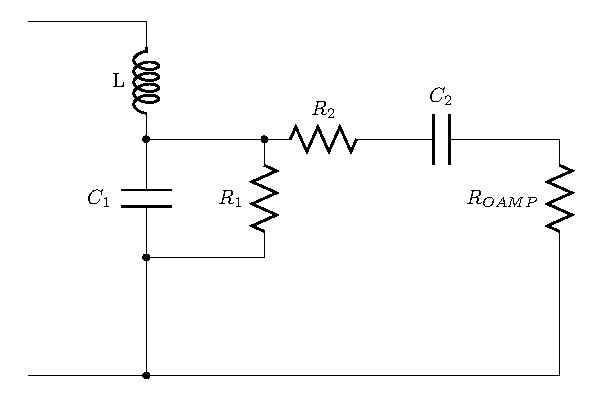
\includegraphics[width=0.48\textwidth]{images/Bandpass/half}
    \caption{vereinfachte Schaltung des Filters}
    \label{fig:filter_half}
\end{figure}\\
Dabei wurden für die Elemente L = 5.4 $\mu$H, $C_1$ = 47 pF, $R_1$ = 390 $\Omega$, $R_2$ = 24 $\Omega$ und $C_2$ = 235 pF bestimmt.
Diese Schaltung betrachtet jedoch nur eine Hälfte des Filters, wodurch die Werte für $L$ und $C_2$ der Schaltung wie folgt berechnet werden.
\begin{align*}
L=&\frac{L}{2}\\
C_2=&2\cdot C_2
\end{align*}
\clearpage
\begin{figure}[!h]
        \centering
        \begin{subfigure}[b]{0.48\textwidth}
                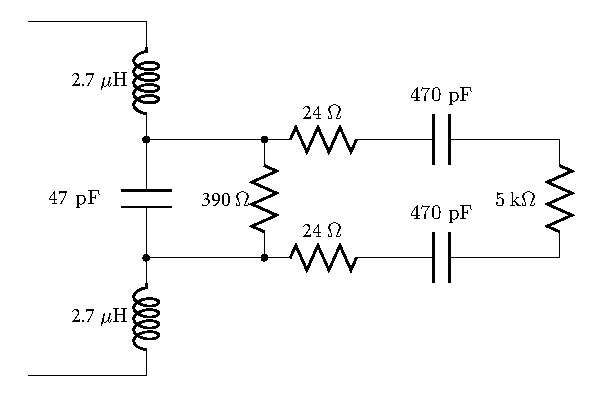
\includegraphics[width=\textwidth]{images/Bandpass/full}
	    		\caption{realisierbare Schaltung des Filters}
	    		\label{fig:filter_full}
        \end{subfigure}%
        ~ %add desired spacing between images, e. g. ~, \quad, \qquad, \hfill etc.
          %(or a blank line to force the subfigure onto a new line)
        \begin{subfigure}[b]{0.48\textwidth}
        	\includegraphics[width=\textwidth]{images/Bandpass/Bandpass}
		    \caption{Verhalten des Filters}
		    \label{fig:filter_verhalten}
        \end{subfigure}
        \caption{realisierbarer Filter}\label{fig:filter_final}
\end{figure}
Daraus ergibt sich die Schaltung aus \autoref{fig:filter_full}, welche mit beziehbaren Kaufteilen realisiert werden kann und dabei eine Filtercharakteristik nach \autoref{fig:filter_verhalten} aufweist. Dabei liegt die untere Grenzfrequenz $f_L$ bei 120 \ac{khz} und die obere Grenzfrequenz $f_H$ bei 13 \ac{mhz} wobei bei 1 \ac{mhz} die minimale Dämpfung von 0,1 dB vorherrscht.\\
Verstärkungen konnten jedoch im Bereich von 1,5 \ac{mhz} bis 10,5 \ac{mhz} erreicht werden.
\subsection{analoge Vorverstärkung}
Der Verstärkungsfaktor ist maßgeblich für das Signal-Rausch-Verhältnis und muss somit möglichst groß dimensioniert werden. Es wurde sich für einen differenziellen Verstärker von Analog Devices mit der Bezeichnung AD8351 entschieden\cite{ad8351}, bei dem die Verstärkung zwischen 0 und 26 dB justiert werden kann, was einen Spannungsverstärkung von 0 bis rund 20 mal dem Eingangssignal entspricht.\\
Damit der ideale Faktor bestimmt werden kann, wurde festgelegt, dass bei einen 50 $\Omega$ Eingangswiderstand ein Eingangssignal von 100 mVpp den gesamten Messbereich des 14-Bit \ac{adc}s abdeckt. Da der Eingangsbereich des \ac{adc}s auf 2 Vpp festgelegt ist, muss der Verstärkungsfaktor 20 betragen um den gesamten Bereich auszusteuern. Nach \autoref{fig:graph_gain} erkennt man, dass der differentielle Verstärker noch eine Dekade über der Nutzfrequenz konstant verstärkt. Daher muss der Lastwiederstand R$_L$ und der Verstärkungswiderstand R$_G$ näher betrachtet werden. Der \ac{adc} besitzt einen hochohmigen Eingang mit 7 k$\Omega$ wodurch ein Verstärkungswiderstand R$_G$ von 10 $\Omega$ oder kleiner benutzt werden sollte.
Da Bauelemente der E12 Reihe eine fertigungsbedingte absolute Toleranz von 5 $\%$ aufweisen, wurde sich für einen 8,2 $\Omega$ Widerstand für R$_G$ entschieden, um einen Verstärkungsfaktor von 20 zu erreichen.\\
Da jeder Verstärker ein Eigenrauschen aufweist und eine zu hohe Verstärkung das Signal-Rausch-Verhältnis verschlechtern kann, muss bei der Inbetriebnahme des gesamten Receiversmoduls der Verstärkungsfaktor für ein optimales Signal-Rausch-Verhältnis angepasst werden.
\begin{figure}[h!]
	\centering
	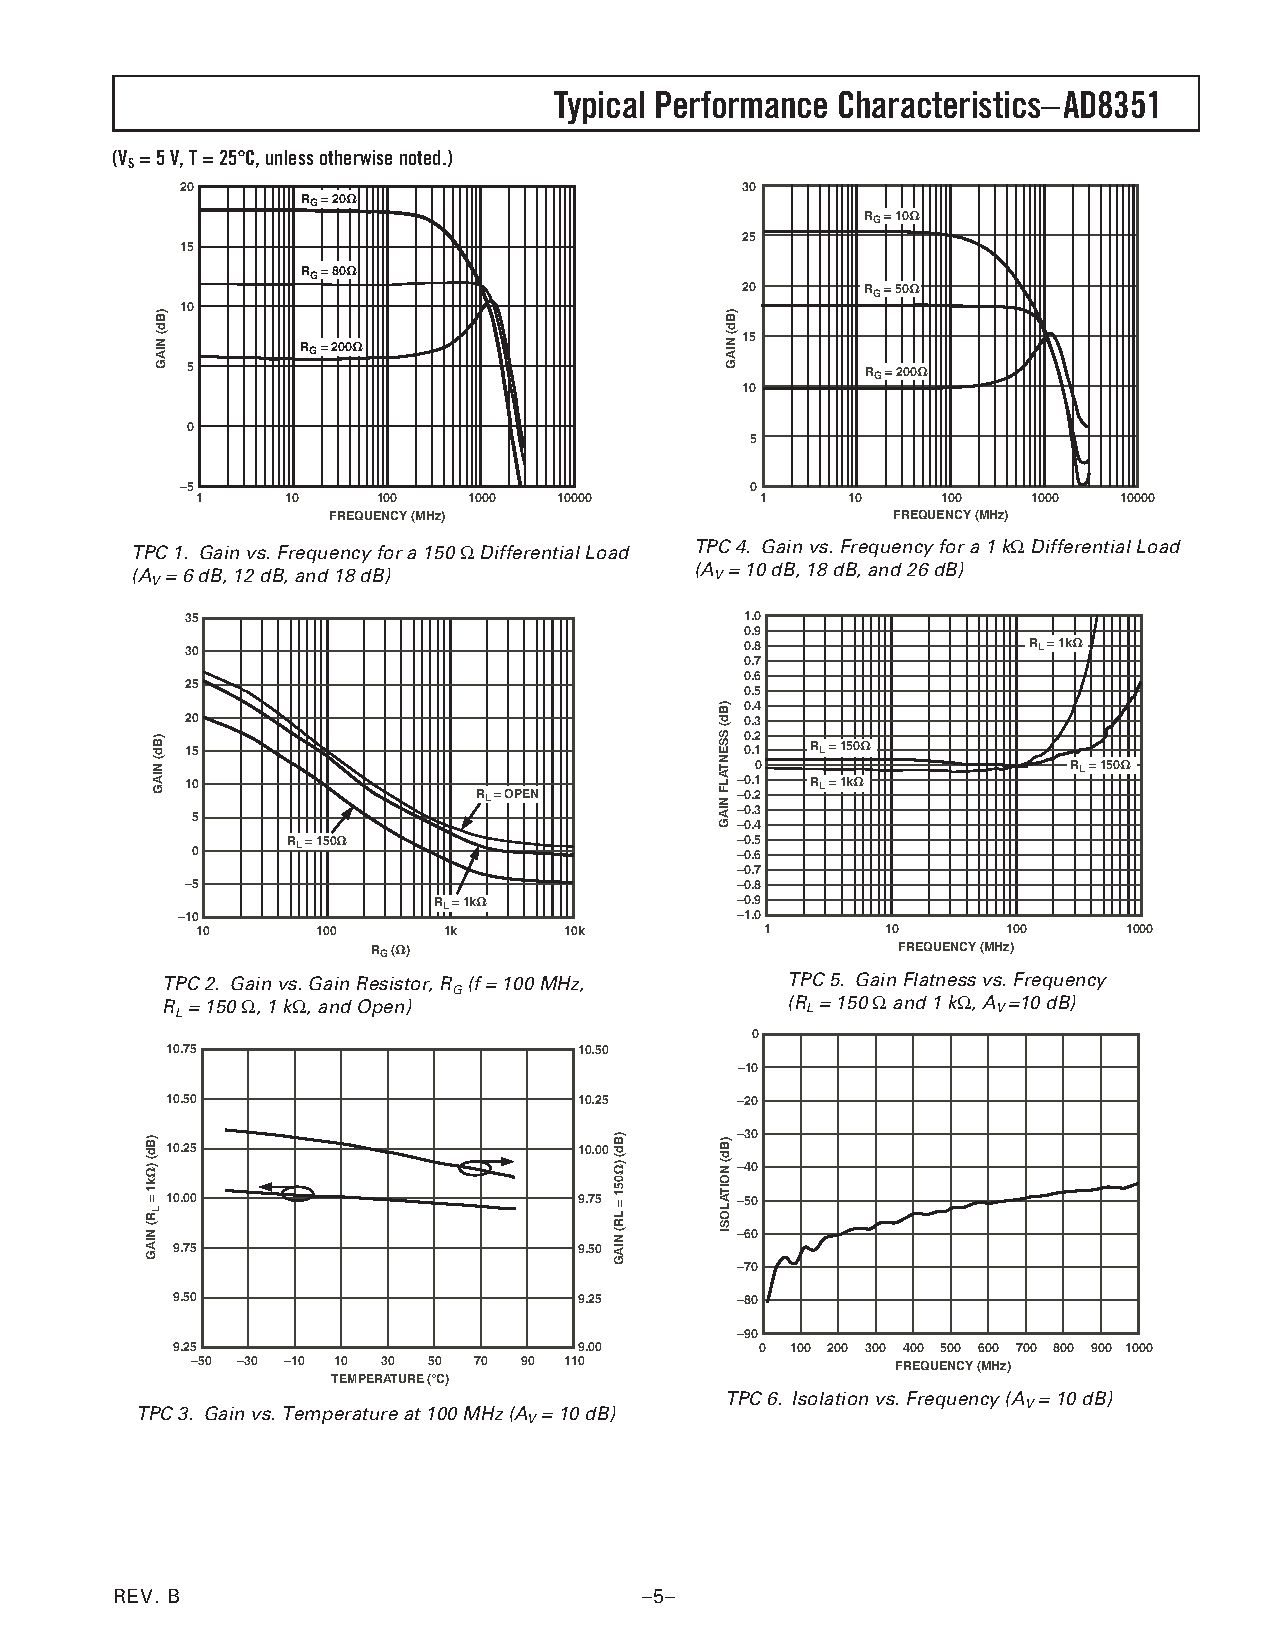
\includegraphics[width=1.0\textwidth, trim=20mm 180mm 15mm 30mm, clip=true]{images/Gain}
	\caption[Verstärkung in Abhängigkeit von Differenzieller Last, Frequenz und Verstärkungs-widerstand R$_G$]{Verstärkung in Abhängigkeit von Differenzieller Last, Frequenz und Verstärkungswiderstand R$_G$\cite[p. 7]{ad8351}}
	\label{fig:graph_gain}
\end{figure}
\newpage
\subsection{Digitalisierung}
Für die Diskretisierung des Signals und für dessen Weiterverarbeitung wird eine Analog-Digital-Wandlung benötigt. Da das Signal differenziell vorliegt, wurde der differenzielle \ac{adc} AD9245 der Firma Analog Devices verwendet, um die Vorteile des differenziellen Signals nicht zu verlieren.\cite{ad9245} \textbf{[REF! EMV / DIFF / SINGLE-ENDED]}\\
Dieser erzielte in den vorangegangen Arbeiten bereits ausreichende Messergebnisse. Dabei ist zu erwähnen das dieser 64 \ac{mhz} High-Speed \ac{adc} das Nyquistkriterium um ein 4-faches der maximalen Trägerfrequenz (8 \ac{mhz}) überschreitet. Dies wird wie in \textbf{[REF]} beschrieben für die Quadraturdemodulierung benötigt um eindeutige Aussagen über die Phase des Signals zu erhalten. Bei 4 Diskretisierungen pro Periode, also dem 2-fachen Nyquistkriterium, kann nicht garantiert werden, dass die maximale Auslenkung sowie die Nulldurchgänge digitalisiert werden, wodurch ein Quantisierungsfehler die Folge ist. Bei den Trägerfrequenzen von 2 und 4 \ac{mhz} kann zudem ein Oversampling mit 32 und 16 Diskretisierungen pro Periode erfolgen, wodurch für diese Frequenzen detailliertere Aussagen getroffen werden können.\\
Da auch in tieferen Blutgefäßen Aussagen über die Teilchengeschwindigkeiten getroffen werden müssen, wird eine hohe dynamic range benötigt, welche nur durch eine erhöhte Bitanzahl erzielt werden kann. Dabei wird folgende Formel mit der Bitanzahl N verwendet, um die Auflösung des \ac{adc}s zu erhalten, wobei positive sowie negative Amplituden digitalisiert werden sollen.\cite[p. 59]{lattice_adc}
\begin{equation}
V_{resolution} =\pm\frac{1}{2}\Delta V_{IN}/2^{N}\label{eq:adc_res}
\end{equation}
Nach \autoref{eq:adc_res} erreicht man theoretisch mit 14 Bit und einen Eingangsbereich von 1 Vpp eine Auflösung von 122 $\mu$V und bei 2 Vpp von 244 $\mu$V. Bei 12 Bit hingegen jedoch nur 488 $\mu$V bei 1 Vpp Range und 977 $\mu$V bei 2 Vpp. Somit ergeben 2 bit mehr eine 4-fach bessere Genauigkeit wodurch sich aus diesen Grund für einen 14 bit \ac{adc} entschieden wurde. Jedoch wird der AD9245 mit einen Eingangsbereich von 2 Vpp betrieben um das bestmögliche \ac{snr} zu erreichen.\cite[p. 18]{ad9245}\\
Um Störungen des analogen Bereiches zu vermeiden, wurde das Ringing \textbf{[REF RINGING]} der Busausgänge durch Serienterminierung reduziert, wodurch die Signalintegrität in diesen Bereich gesteigert wird. Zudem wurde ein Tiefpass 2. Ordnung für die Stromversorgung vorgesehen, um den \ac{adc} von anderen \ac{ic}s in diesem Stromkreis induktiv zu entkoppeln und periodische Stromspitzen in der Spannungsversorgung zu vermeiden.
%
%
%
\section{Steuerung und Demodulierung}
Für die Applikation der Emboliedetektion muss die Peripherie nach Bedarf parametriert und angesteuert werden, damit die zeitkritische digitale Demodulierung korrekt arbeiten kann. Dafür wird ein Zustandsautomat benötigt, welcher nach parametrierten Zeiten einen Burst, die Digitalisierung sowie Demodulierung für den parametrierten Zeitraum ansteuert. Zudem müssen die modulierten Daten zwischengespeichert werden, wobei sich ein \ac{ram} \ac{resp} ein \ac{fifo} eignet.\\
Für die benötigte Funktionalität wurde das \ac{cpld} MachXO2\SymbTM der Firma Lattice Semicondutors Corp. verwendet\cite{machxo2}, da in der vorangestellten Arbeit die logischen Verknüpfungen des \ac{cpld}s MachXO\SymbTM ausgeschöpft waren. Somit wurde als Konsequenz die größtmögliche Version vorgesehen, um die Entwicklungsphase nicht zu stören und Implementierungen wie einen digitalen Hochpass zu integrieren.
\begin{figure}[h!]
	\centering
	\includegraphics[page=11,width=1.0\textwidth, trim=28mm 89mm 38mm 35mm, clip=true]{images/pcb/new.PDF}
	\caption{Abstrahierung der Logik für die Steuerung und Demodulierung der Doppler-Kernapplikation}
	\label{fig:layer_cpld}
\end{figure}\\
Die Logik wurde in Module untergliedert um Änderungen sowie Modultests zu realisieren. Dabei wurde die Abstrahierung der Logik an einen Zustandsautomaten angelegt, welcher über Register parametriert ist. Um die Register zu schreiben und zu lesen wurde ein \ac{spi} vorgesehen, da dieser durch Schieberegister angenehm in Logik abgebildet werden kann. Um die demodulierten Daten möglichst schnell zu transferieren wurde sich für eine parallele Schnittstelle entschieden, welche in der Logikschicht Kommunikation abgebildet wurde. Um die einzelnen Schichten zu Testen wurde weiterhin für jede Schicht eine Testbench geschrieben, welche als Validierung der einzelnen Schichten dient. Somit konnten Fehler in der Logik schnell erkannt werden, was die Entwicklungszeit reduzierte.
Die nachgestellten Abschnitte beschreiben die Funktionalität der einzelnen Logikschichten genauer.
\subsection{Logikschicht Zustandsautomat}\label{subsec:fsm}
\begin{figure}[!h]
        \centering
        \begin{subfigure}[b]{0.48\textwidth}
                \includegraphics[page=11,width=\textwidth, trim=169mm 126mm 68mm 35mm, clip=true]{images/pcb/new.PDF}
				\caption{Abstrahierung}
	    		\label{fig:Layer_fsm}
        \end{subfigure}%
        ~ %add desired spacing between images, e. g. ~, \quad, \qquad, \hfill etc.
          %(or a blank line to force the subfigure onto a new line)
        \begin{subfigure}[b]{0.48\textwidth}
        \resizebox{1\textwidth}{!}{%
        	\begin{tikzpicture}[shorten >=1pt,node distance=4cm,on grid,auto] 
\tikzstyle{every lower node part}=[font=\footnotesize]
  \node[circle split,draw]					(q_0)						{$S4$ 	\nodepart{lower}0, 1, 0, 1};
  \node[circle split,draw]							[left =of q_0]		{$State$\nodepart{lower}TX, RX, D, R};
  \node[circle split,draw]					(q_2)	[above of=q_0]		{$S1$ 	\nodepart{lower}0, 1, 0, 0};
  \node[circle split,draw,initial,accepting](q_1)	[left =of q_2]		{$S0$ 	\nodepart{lower}1, 1, 0, 0};
  \node[circle split,draw]					(q_3)   [right=of q_2]		{$S2$ 	\nodepart{lower}0, 1, 1, 0};
  \node[circle split,draw]					(q_4)   [right=of q_0]		{$S3$ 	\nodepart{lower}0, 1, 0, 0};

	\path[->]
    (q_1) edge	[bend left]		node {$[Cnt==S0V]$}	(q_2)
    (q_2) edge	[bend left]		node {$[Cnt==S1V]$}	(q_3)
    (q_3) edge	[bend left]		node {$[Cnt==S2V]$}	(q_4)
    (q_4) edge	[bend left]		node {$[Cnt==SRV]$}	(q_0);
%    
%	(q_1) edge	[loop left]		node[text width=1.5cm, align=center] {$Cnt<V(S1)$}	(q_1)
%    (q_1) edge	[bend left]		node[text width=1.5cm, align=center] {$Cnt=V(S1)$}	(q_2)      
%	(q_2) edge	[loop above]	node {$Cnt<V(S2_0)$}(q_2)
%    (q_2) edge					node {\ldots}	(q_3)
%	(q_3) edge	[loop above]	node {$Cnt<V(S2_n-1)$}(q_3)
%    (q_3) edge	[bend left]		node[text width=1.5cm, align=center] {$Cnt=V(S2_n)$}	(q_4)
%    (q_4) edge	[loop right]	node[text width=1.5cm, align=center] {$Cnt<V(S3)$}	(q_4);%end path
%    (q_4) edge	[bend left]		node[text width=1.5cm, align=center] {$Cnt=V(S3)$}	(q_5)
%    (q_5) edge	[loop below]	node {$Cnt<V(S4)$}	(q_5)
%    (q_5) edge	node[text width=1.5cm, align=center] {$Cnt=V(S4)$}	(q_0); %end path

	\path[->]
    (q_0) edge	[bend left]		(q_1)
    (q_2) edge	[bend left]		node[pos=0.25,  above] {$\overline{EN}$} (q_1)
    (q_3) edge	[bend left]		node[pos=0.25,  above] {$\overline{EN}$} (q_1)
    (q_4) edge					node[pos=0.25,  above] {$\overline{EN}$} (q_1);
%    (q_5) edge	[bend right]	node {$\overline{E}$}(q_0);
    
%\draw[decorate,decoration={brace,raise=60pt}, thick] ($(q_2.north west)+(-0.5,0)$)--($(q_3.north east)+(0.5,0)$);

%\path ($(q_3.north west)+(-1.5,2.4)$) node[text width=7cm, align=center] {Anzahl n der Samplevolumes 1 \& 2};
    \end{tikzpicture}
    }
    \caption{Zustände und Weiterschaltbedingungen}
    \label{fig:fsm_function}
    \end{subfigure}
    \caption{Modul Zustandsautomat}
    \label{fig:fsm}
\end{figure}

Für die zeitlich wiederkehrende Ansteuerung der Peripherie wird ein Moore-Zustandsautomat genutzt, wodurch die Ausgabe durch den aktuellen Zustand definiert ist. Dabei handelt es sich prinzipiell um einen Automaten, welcher seine Parameter mit einen Zählwert eines aufwärts zählenden Zählers vergleicht. Wenn der Wert des Zählers dem Wert des Parameters entspricht, schaltet der Automat in den nächsten Zustand.\\
Somit kann eine Aktivierung der Peripherie wie in \autoref{sec:pw} beschrieben erreicht werden. Dabei ist zu beachten, dass die Werte des Zählers und die Parameterwerte der einzelnen Zustände mit der gleichen Frequenz arbeiten.
Als Beispiel soll hier die Erzeugung der \ac{prf} genannt werden. Diese benötigt bei einer Zählfrequenz von 64 \ac{mhz} 6400 Flanken um einen neuen Burst zu generieren. Bei einer Zählfrequenz von 32 \ac{mhz} hingegen nur 3200 Flanken. Aus diesen Verhalten sowie der erhöhten zeitlichen Auflösung des Zustandsautomaten wurde eine Automatenfrequenz von 64 \ac{mhz} definiert.\\
Der in dieser Arbeit implementierte Zustandsautomat besitzt 5 Zustände, welche durch 4 16-Bit Parameterwerte beschrieben werden. Nach \autoref{sec:pw} wird ein Wert für die Burstlänge, ein Wert für die Pause zwischen Burstende und Demodulierungsanfang sowie ein Wert für die Länge der Demodulierung und ein Wert für die Länge der \ac{prf} benötigt. Diese werden aus den Registern des nachfolgenden \autoref{subsec:cpld_register} den Zuständen zugewiesen, wodurch sich eine Änderung der Parameter sofort auf den Automaten auswirkt. Zudem steuert der Zustandsautomat sich selbst, wobei dieser jedoch durch ein Reset-Impuls in einen definierten Grundzustand versetzt wird und durch ein Enable Signal de- \ac{bzw} aktiviert.\\
Den definierten Zuständen werden Funktionen zugeordnet, wodurch ein Gating der Peripherie erreicht werden kann. Anhand dieser Zuordnung wird die funktionale Ansteuerung der Peripherie zu dieser Logikschicht hinzugefügt, was eine Abbildung der zeitliche Ansteuerung (Gating) und der funktionalen Ansteuerung der Peripherie in einer Schicht zur folge hat. Somit kann der Automat in Verbindung zur ausgegebenen Funktion betrieben und getestet werden, was die Komplexität reduziert und die Inbetriebnahme durch eine Testbench erleichtert.
Die funktionale Ansteuerung betrifft lediglich die Transmitter-, die Receiveransteuerung und die Aktivierung der Demodulierung. Dabei wird ein Frequenzteiler für Generierung der Träger- und Diskretisierungsfrequenz genutzt, welcher durch einen Wert aus einen Register der nachfolgenden Memorymap parametriert wird. Die Demodulierung wird durch ein High-Level aktiviert und durch ein Low-Level deaktiviert sowie resetet.
\subsection{Logikschicht Memorymap}\label{subsec:cpld_register}
\begin{figure}[!h]
	\centering
	\includegraphics[page=11,width=0.48\textwidth, trim=111mm 118mm 127mm 43mm, clip=true]{images/pcb/new.PDF}
	\caption{Modul MemoryMap}
	\label{fig:layer_map}
\end{figure}
Die 16-Bit Werte für die Zustände des Zustandsautomaten aus \autoref{subsec:fsm} müssen effizient geschrieben und gelesen werden. Zudem werden Einstellungen wie Trägerfrequenz, Transmitter an/aus, Receiver an/aus, Zustandsautomat an/aus und Anzahl der Bytes pro Frame benötigt, welche gesetzt und gelesen werden müssen. Aus diesen Sachverhalten ist ein 16-Bit breiter und 12 Byte tiefer Speicher erstellt wurden, welcher nachfolgend in \autoref{tab:map_address} und \autoref{tab:map_params} beschrieben ist. So kann durch Anwahl der Adresse das Register geschrieben oder gelesen werden.
\newpage
\begin{table}[h]
\centering
\caption{Bedeutung der Speicheradressen}
\label{tab:map_address}
\begin{tabular}{|c|l|}
\hline 
Adresse & Beschreibung\\  \hline
0x0000 & Endzählwert der Bursttiefe\\ \hline
0x0001 & Startzählwert der Demodulierung\\ \hline
0x0002 & Endzählwert der Demodulierung\\ \hline
0x0003 & Zählwert für Reinitalisierung der \ac{prf}\\ \hline
0x0004 & Einstellung für den Zustandsautomaten\\ \hline
0x0005 & Anzahl der Bytes pro Frame\\ \hline
\end{tabular} 
\end{table}

\begin{table}[h]
\centering
\caption{Bedeutung der Adressparameter}
\label{tab:map_params}
\newcommand{\celling}[2]	{\multirow{#2}{*}{\hfil #1}}
\begin{tabular}{|p{3cm}|c|p{4cm}|l|}
\hline 
Adresse  & Bit & Funktion & Wert \\  \hline
\celling{0x0000 bis 0x0003}{2} & \celling{[15:0]}{2} & Vergleichswert für Zustandsweiterschaltung & \celling{0 bis $2^{16}$}{2} \\ \hline
\celling{0x0004}{2} & \celling{[0]}{2} 		& \celling{TX de-/aktiviert}{2}	& 1 := aktiviert \\	&&&0 := deaktiviert\\ \hline
\celling{0x0004}{2} & \celling{[1]}{2} 		& \celling{RX de-/aktiviert}{2}	& 1 := aktiviert \\	&&&0 := deaktiviert\\ \hline
\celling{0x0004}{2} & \celling{[4]}{2}		& \celling{Zustandsautomat}{2}	& 1 := aktiviert \\	&&&0 := deaktiviert\\ \hline
%0x0004 & [7:5]		& GateDivider & 0 \ldots 7 \\ \hline
%0x0004 & [15:8]	& Sampevolume Länge & 0 \ldots 255 \\ \hline
\celling{0x0004}{3} & \celling{[15:14]}{3} 	& \celling{Trägerfrequenz}{3}			 & 11 := 8 MHz \\		&&& 10 := 4 MHz	\\	&&& 01 := 2 MHz\\ \hline
\celling{0x0005}{2} & \celling{[15:0]}{2} & Vergleichswert für Zustandsweiterschaltung & \celling{0 bis $2^{16}$}{2} \\ \hline
\end{tabular} 
\end{table}
\newpage
\subsection{Logikschicht Kommunikation}
\begin{figure}[h!]
	\centering
	\includegraphics[page=11,width=0.48\textwidth, trim=58mm 99mm 185mm 53mm, clip=true]{images/pcb/new.PDF}%28 links
	\caption{Modul Kommunikation}
	\label{fig:layer_com}
\end{figure}
Diese Schicht wurde erstellt, um die Komplexität der Kommunikation auf ein Minimum zu reduzieren. Dabei wurden die Information genutzt, dass die Parametrierung des Zustandsautomaten aus \autoref{subsec:fsm} mehrere Adressen benötigt und gelesen werden sollten um den Benutzer Informationen der aktuellen Einstellung zur Verfügung zu stellen. Die Datenübertragung der Parameter der Register wird über ein \ac{spi} realisiert, welche in \autoref{subsec:spi} nähe beschrieben wird. Durch den Vollduplexmodus der Schnittstelle wurde ein Burstmodus implementiert, wodurch ein sequenzielles Lesen und Schreiben mehrere Adressen ohne erneute Anwahl der nächsten Adresse ermöglicht wird.\\
Zudem wurde ein FlipFlop integriert, welches durch eine 16-Bit Übertragung gesetzt oder gelöscht werden kann. Dieses wird für die parallele Datenübertragung, welche in \autoref{subsec:interface_parallel} näher beschrieben ist, benötigt damit der ARM\SymbReg Cortex\SymbReg-M die Daten nach Bedarf Pullen\footnote{abholen von Paketen nach Bedarf} kann. Dieser FlipFolp wird nach Beendigung einer parallelen Datenübertragung gelöscht, wodurch ein erneuter Datentransfer blockiert wird. 
Bei jeder negativen Flanke des DATA\_CLK Signals wird zudem die Adresse der zu übertragenden Daten aus der Speicherschicht weiter geschaltet, wodurch ein Streaming der Daten ermöglicht wird.\\
Nachfolgend werden die Befehle mit möglichen Kombinationen der Datenübertragungen sowie deren sequenzieller Abläufe beschrieben.
\begin{longtable}{|l|c|c|c|c|}
\textbf{Operation} 	& \textbf{Befehl} & \textbf{Adressword} & \textbf{Dummyword} & \textbf{Datenword} \kill
\caption{\ac{spi} Befehle\label{tab:spiBefehle}}\\
\hline

\endfirsthead
\caption[]{(Fortsetzung \ac{spi} Befehle)}\\
\hline
\textbf{Operation} 	& \textbf{Befehl} & \textbf{Adressword} & \textbf{Dummyword} & \textbf{Datenword} \\\hline \endhead
\textbf{Operation} 	& \textbf{Befehl} & \textbf{Adressword} & \textbf{Dummyword} & \textbf{Datenword} \\\hline
Datentransfer an 	& 0x0006 & - & - & -\\\hline
Datentransfer aus	& 0x0004 & - & - & -\\\hline
Speicher schreiben	& 0x0002 & 1 & - & 1+\\\hline
Speicher lesen		& 0x0008 & 1 & 1 & 1+\\\hline
\end{longtable}

\begin{figure}[h!]
\centering
\begin{subfigure}[b]{0.48\textwidth}
	\centering
   \begin{tikztimingtable}[timing/d/background/.style={fill=white},
   timing/lslope=0.2]
	 		MOSI & U u 4D{0x0006} u U  \\
	 		MISO & U u 4D{ID} u U  \\
	 		CS 	 & H 5L H \\
\end{tikztimingtable}
	\caption{Datentransfer aktivieren}
   \label{fig:com_on}
\end{subfigure}
\begin{subfigure}[b]{0.48\textwidth}
	\centering
   \begin{tikztimingtable}[timing/d/background/.style={fill=white},
   timing/lslope=0.2]
	 		MOSI & U u 4D{0x0004} u U  \\
	 		MISO & U u 4D{ID} u U  \\
	 		CS 	 & H 5L H \\
\end{tikztimingtable}
	\caption{Datentransfer deaktivieren}
   \label{fig:com_off}
\end{subfigure}

\begin{subfigure}[b]{0.48\textwidth}
	\centering
   \begin{tikztimingtable}[timing/d/background/.style={fill=white},
   timing/lslope=0.2]
	 		MOSI & U u 4D{0x0002} 4D{Adresse} 4D{Daten}4D{...} u U  \\
	 		MISO & U u 4D{ID} 4Z 4D{Daten}4D{...} u U  \\
	 		CS 	 & H 17L H \\
\end{tikztimingtable}
	\caption{Speicher schreiben}
   \label{fig:com_read}
\end{subfigure}
\begin{subfigure}[b]{0.48\textwidth}
	\centering
   \begin{tikztimingtable}[timing/d/background/.style={fill=white},
   timing/lslope=0.2]
	 		MOSI & U u 4D{0x0008} 4D{Adresse} 4D{Dummy} 4D{Daten}4D{...} u U  \\
	 		MISO & U u 4D{ID} 8Z 4D{Daten}4D{...} u U  \\
	 		CS 	 & H 21L H \\
\end{tikztimingtable}
	\caption{Speicher lesen}
   \label{fig:com_read}
\end{subfigure}
\caption{\ac{spi} Datenübertragung}
\end{figure}

\subsection{Logikschicht Signalverarbeitung}
\begin{figure}[h!]
	\centering
	\includegraphics[page=11,width=0.48\textwidth, trim=169mm 96mm 66mm 74mm, clip=true]{images/pcb/new.PDF}%28 links
	\caption{Modul Signalverarbeitung}
	\label{fig:layer_demod}
\end{figure}
Um das diskretisierte Signal für die Applikation nutzen zu können wird zunächst der Offset durch einen Hochpass entfernt, welcher in \autoref{sec_digHP} näher beschrieben wird. Der Offset entsteht bei der Digitalisierung durch die integrierte switched-capacitor Schaltung des \ac{adc}s, sowie durch eine Phasenverschiebung des differenziellen Signals, welche die Folge von Toleranzen der \ac{smt} Bauelemente ist. Anschließend folgt die Quadraturdemodulierung, welche in \autoref{sec:demodulate} beschrieben wird. Dies beschreibt die grundsätzliche Funktionalität sowie den Signalfluss dieser Logikschicht.\\
Die Logik des Quadraturdemodulators benötigt eine Sinus-Cosinus Tabelle für die Multiplizierung des Signals. Dabei wurde sich für eine 8-Bit genaue Tabelle entschieden, welche mit der Trägerfrequenz rotiert. Darunter ist zu verstehen, dass bei 8 Diskretisierungen pro Periode des Signals die Tabelle genau 8 Werte für eine Periode beinhaltet. Zudem werden für die Multiplikation des diskretisierten Signals mit den Sinus- und Cosinuswerten zwei Multiplizierer benötigt. Da bei einer Multiplikation von 14-Bit und 8-Bit Werten ein 22-Bit Wert entsteht, muss nach der Multiplikation der Wert in einen 32-Bit Wert umgewandelt werden, damit bei der nachgestellten Addition des Tiefpasses mögliche Überläufe vermieden werden können.\\
Durch die Limitierung der Kernfrequenz des Systems auf die maximale Samplingfrequenz von 64 \ac{mhz} muss bei der weiteren Verarbeitung auf das Verhalten der Register geachtet werden. Diese Flip-Flops schalten jeweils bei positiver Flanke weiter, worauf hin zwei Addierer pro Quadratur- und Inphase benötigt werden, damit ein Datenverlust bei Reinitialisierung des Tiefpassfilters\footnote{Startwert der Addition muss auf 0 gesetzt werden, um einen Offset zu vermeiden} verhindert wird. 
\subsection{Logikschicht Storage}
\begin{figure}[h!]
	\centering
	\includegraphics[page=11,width=0.48\textwidth, trim=111mm 89mm 127mm 81mm, clip=true]{images/pcb/new.PDF}%28 links
	\caption{Modul Storage}
	\label{fig:layer_fifo}
\end{figure}
Diese Schicht wurde implementiert, damit die Speicherung der demodulierten Daten mit der dafür benötigten Ansteuerung und Flags vereinfacht wird. Für die Speicherung wird ein \ac{fifo} mit dualen Takt genutzt, welches von Lattice Semicondutors Corp. für den MachXO2\SymbTM implementiert wurde und als parametriertes Modul in der IPexpress Bibliothek von \nameref{subsub:diamond}\SymbTM bereitgestellt wird. Es wurde sich dabei für eine Implementierung mit den embedded RAM des \ac{cpld}s entschieden, da dieser Bereich in Hinblick auf \ac{lut}s zwar langsamer, jedoch aber Platzsparender ist. Zudem wurde die Speicherung der Daten an die des ARM\SymbReg Cortex\SymbReg-M auf Big Endian angepasst, um Fehler zu vermeiden. Die Eingangsdatenbreite wurde mit 64-Bit (2x32-Bit) und die Ausgangsdatenbreite mit 8-Bit definiert. Somit wird keine zusätzliche Logik für die Reduzierung der Datenbreite benötigt und durch die Aneinanderreihung der Daten erfolgt ein sequenzielles auslesen der In- und Quadraturphase Daten.\\
Durch den Ringspeicher mit separaten schreib und lese Takt wird eine Entkopplung der Demodulierung und des Datentransfers zu Verfügung gestellt, wodurch die Komplexität des Systems, Fehler und Datenverluste reduziert werden.
\vfill
\subsection{Logikschicht Testbench}

\newpage
\section{Kommunikation / Datenübertragung}
Dafür wurde in dieser Entwicklungsphase ein asymmetrischer Mehrkern ARM\SymbReg Cortex\SymbReg-M4 der Firma NXP Semiconductors als Schnittstelle zwischen Benutzerinterface und Peripherieansteuerung genutzt, da dieser eine High-Speed USB 2.0 Schnittstelle mit einer theoretischen Datenrate von 480 mbit/s zu Verfügung stellt.
\subsection{Hardware}
\subsection{Software}
\newpage
\section{Visualisierung}
\subsection{Algorithmus}
\newpage
\subsection{\ac{gui}-Beschreibung}
\newpage
\subsection{Programmablauf}
\newpage